\section{UNE line selection}
\label{sec:uneselect}

\subsection*{Storing and using line selections}

Static calibration files containing UNE line lists are distributed with the
pipeline, and are named like \linebreak \verb#lines_u_redman_H1575.fits#. These
are the input to \verb#cr2res_cal_wave# or \verb#cr2res_util_wave# and contain a
subset of lines from the full catalogs by \cite{2018A&A...618A.118S} and
\cite{2011ApJS..195...24R} which has been manually selected to only contain
usable lines for the current setting.

The raw catalogs are part of \emph{cr2rep}, as txt-files in the subdirectory
\emph{catalogs/}, containing the wavelength and strength of the lines. In the
subdirectory \emph{selections/} there are further txt-files, one for each
setting. They contain one \emph{usable wavelength region} per line, i.e. start
and end wavelength between which there are only usable lines in the full
catalog. This can be a single line, a group of lines, or a whole detector-order; depending on how well the catalog locally matches the obtained spectra.

The recipe \verb#cr2res_util_genlines# then takes the catalogs and selection files to generate the FITS-files above.

The following describes how to go about selecting lines. This might become necessary when the UNE lamp is exchanged\footnote{Yes, they can be surprisingly different.} or has aged, or when for some other reason the cross-correlation  between spectrum and catalog no longer gives a reliable zero-point to the wavelength solution.

\subsection*{Selecting lines}


\begin{figure}[ht]
    \begin{center}
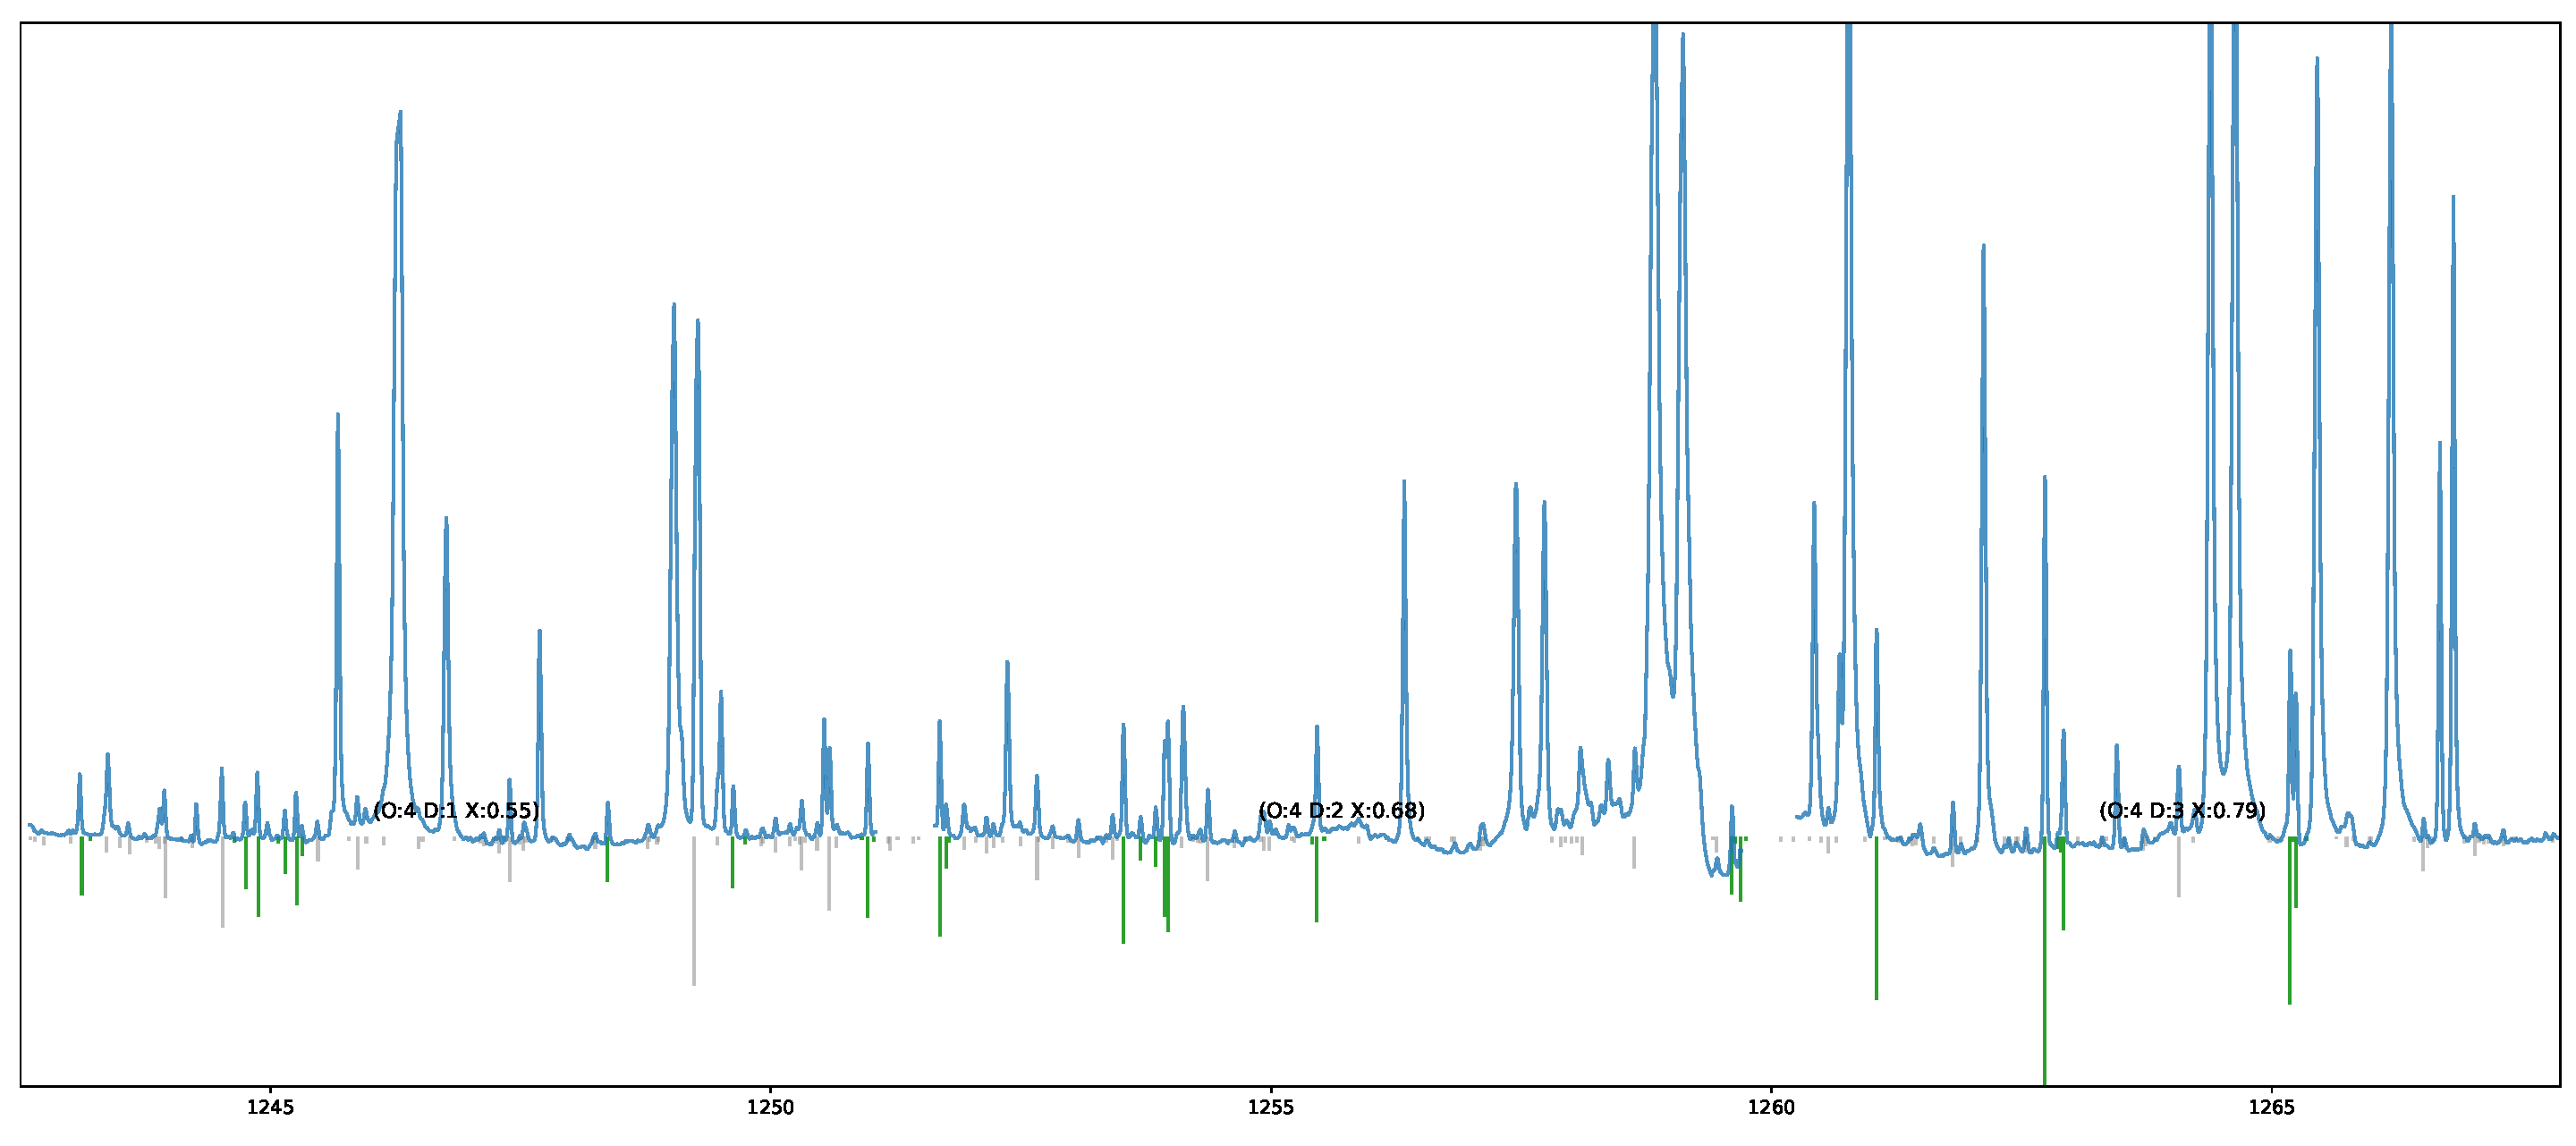
\includegraphics[width=1.25\linewidth, angle=90]{linesel_examp.pdf}
\end{center}
\caption{An example of a UNe spectrum in setting J1228. The catalog lines are
 plotted upside down, in green the selected lines, in gray the not-selected
 ones. }
\label{fig:linesel}
\end{figure}


Earlier attempts had been made to select lines by objective criteria, or by
analyzing spectra from other lamps or instruments. In practice however, it
turned out that these were both insufficient in wavelength coverage and
``cleanliness'' of the lines (in terms of blends, ghosts etc.). 

What worked well when we started to calibrate \instrument , was to visually
compare the spectra to the catalog in a plot like Fig.~\ref{fig:linesel}. It
becomes apparent quickly from the relative line strengths, which lines in the
spectrum are the catalog lines.

There are several sources of ambiguity and things to keep in mind when selecting lines:

\begin{itemize}
    \item There are lines in the spectrum that are not in the catalogs. This obviously is true for the strong Ne and Ar lines, but also for plenty of weak lines.
    \item Not all lines in the catalogs are present in the spectra, even among the stronger catalog lines.
    \item The default method applied by the wavecal recipes is cross-correlation with a synthetic spectrum that gets generated from the selected lines. It therefore makes sense to select lines with comparable strengths within the same detector order. At least avoid the case of a single line dominating the correlation.
    \item This is not possible for all wavelength regions. Especially in the K-band, lines become so sparse that you have to take what you get.
    \item Blended lines should be avoided, if possible. When adjacent lines are both in the catalog, with matching relative strengths, they can usually be included.
\end{itemize}


Fig.~\ref{fig:linesel} was made with the script \linebreak
\verb#cr2res_show_spec_catal.py# that is included in the pipeline source code,
subdirectory \emph{tools/}. It provides a rudimentary user interface that allows
to print the wavelength under the cursor, thereby writing the selection file;
see source code for details. Of course, many other tools can be used to do
the simple task of plotting and reading-off wavelengths.